\documentclass{beamer-control}
\usepackage{beamer-control-singlefile}
\INCLUDEONLY{The Nyquist Criterion}
\begin{document}
\CONCEPT{The Nyquist Criterion}

\begin{SUMMARY}
\begin{itemize}
\item Nyquist plot
\item Nyquist criterion
\end{itemize}
\vfill References:
\begin{itemize}
\item \astrom{§10.2}
\end{itemize}
\end{SUMMARY}



\SUBCONCEPT{Nyquist plot}

\begin{frame}{Frequency response graphically}
\begin{itemize}
\item The dynamics of a linear system may be represented by its frequency response and graphically illustrated by a Bode plot
\item We may also graphically represent the frequency response on one graph by using a Nyquist plot, plotted on the complex plane
\item The Nyquist plot of a loop transfer function $L(s)$ is formed by tracing $s\in\mathbb{C}$ around the Nyquist contour $\Gamma$ (given by the imaginary axis combined with an arc at infinite connecting the endpoints of the imaginary axis)
\item At any point on the Nyquist plot corresponding to a frequency $s=i\omega$, the distance away from the origin gives the magnitude of the loop transfer function $L(s)$ and the angle with the imaginary axis gives the phase
\end{itemize}
\end{frame}


\begin{frame}{Nyquist plot}
\begin{figure}
	\centering
	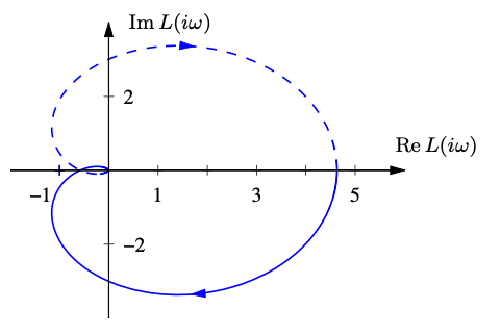
\includegraphics[width=0.9\linewidth]{figure10.5}
	\\
	\textbf{Figure 10.5:} Nyquist plot for a third-order transfer function.
\end{figure}
\end{frame}


\SUBCONCEPT{Nyquist criterion}

\begin{frame}{Condition for stability}
	\textbf{Nyquist criterion}
\begin{itemize}
\item Let $L(s)$ be the loop transfer function for a negative feedback system and assume that $L$ has no poles in the closed right half-plane expect possible at the origin
\item Then the closed loop system \[G_{cl}=\frac{L(s)}{1+L(s)}\]
is stable if and only if the image of $L$ along the closed contour $\Gamma$ has no net encirclements of the critical point $s=-1$
\item The number of encirclements is called the winding number
\item This criterion tells us how the stability of a system is influenced by changing the controller parameters
\end{itemize}
\end{frame}


\begin{frame}{Example}
\begin{itemize}
	\item Consider the transfer function 
	\[L(s) = \frac{k}{s(s+1)^2}\] 
	representing a third-order system with a pole at the origin with nominal gain value $k=1$
	\item The system has a single pole at $s=0$ and a double pole at $s=-1$
	\item The Bode plot thus has the slope $-1$ for low frequencies, and at the double pole the slope changes to $-3$
	\item The phase curve starts at $-90^\circ$ for low frequencies, is $-180^\circ$ at $\omega=1$ and is $-270^\circ$ at high frequencies
\end{itemize}
\end{frame}


\begin{frame}{Example continued}
	\begin{itemize}
		\item The Nyquist curve intersects the negative real axis at $\omega=1$ with $L(i)=-0.5$ for $k=1$
		\item The Nyquist curve only encircles the critical point $s=-1$ when the gain is $k\geq 2$ as $L(i)=-\tfrac{k}{2}$
	\end{itemize}
\begin{figure}
	\centering
	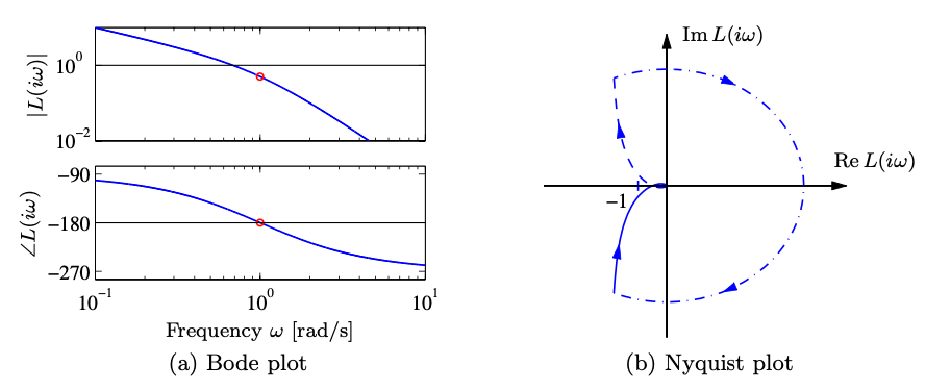
\includegraphics[width=0.9\linewidth]{figure10.6}
	\\
	\textbf{Figure 10.6:} Sketching Nyquist and Bode plots.
\end{figure}
\end{frame}

\SUMMARYFRAME
\FINALE

\end{document}
